%%%%%%%%%%%%%%%%%%%%%%%%%%%%%%%%%%%%%%%%%
% Lebenslauf Template
% Based on the provided image example.
% Version 8: Fully Randomized Content
%%%%%%%%%%%%%%%%%%%%%%%%%%%%%%%%%%%%%%%%%

\documentclass[11pt, a4paper]{scrartcl} % Use KOMA-Script, 11pt font, A4 paper

% --- PACKAGE SETUP ---
\usepackage[utf8]{inputenc}          % Input encoding
\usepackage[T1]{fontenc}             % Font encoding
\usepackage[ngerman]{babel}          % German language support
\usepackage{helvet}                  % Use Helvetica-like font (sans-serif)
\renewcommand{\familydefault}{\sfdefault} % Make sans-serif the default
\usepackage{geometry}                % For page margins
\geometry{left=2.5cm, right=2.5cm, top=2.0cm, bottom=2.0cm} % Define margins
\usepackage{graphicx}                % For including images
\usepackage{tabularx}                % For tables with adjusted column widths
\usepackage{array}                   % For advanced table column formatting
\usepackage{multirow}                % For table cells spanning multiple rows (used elsewhere)
\usepackage[dvipsnames]{xcolor}      % For defining custom colors (if needed)
\usepackage{enumitem}                % For customizing lists
\usepackage{ragged2e}                % Provides \RaggedRight and \Centering
\usepackage{calc}                    % Allows calculations for widths

% --- PAGE STYLE --- 
\pagestyle{empty} % No page numbers

% --- KOMA-Script Section Formatting ---
\setcounter{secnumdepth}{0} % Remove default numbering
\RedeclareSectionCommand[
  beforeskip=2.5ex, afterskip=-0.5em, font=\Large\bfseries
]{section}

% --- Custom Command for Sections with Rule ---
\newcommand{\rulesection}[1]{%
    \section*{#1}% KOMA unnumbered section
    \vspace{0.5ex}% Space title-rule
    {\noindent\rule{\linewidth}{0.4pt}}% Rule
    \vspace{2ex}% Space after rule
}

% --- LIST FORMATTING ---
\setlist[itemize]{
  label=\textbullet, leftmargin=1.5em, topsep=0.3ex,
  partopsep=0pt, itemsep=0.2ex, parsep=0pt
}

% --- CUSTOM COMMANDS FOR CV ENTRIES ---
% Standard entry with bullets (Date Centered)
\newcommand{\cvsectionentry}[4]{%
  \par\noindent
  \begin{tabularx}{\linewidth}{@{} >{\Centering\small}p{3cm} @{\hspace{2em}} X @{}} % Date (CENTERED, small) | Details
    #1 & \textbf{#2} \\ % Date | Bold Title
       & #3 \\          % Empty | Subtitle
       & \vspace{0.5ex}% Space before list
         \begin{minipage}[t]{\linewidth}
           \begin{itemize}#4\end{itemize} % List items
         \end{minipage}
  \end{tabularx}%
  \vspace{1.5ex}% Space after entry
}

% Simpler entry without bullets (Date Centered)
\newcommand{\cveduentrysimple}[3]{%
  \par\noindent
  \begin{tabularx}{\linewidth}{@{} >{\Centering\small}p{3cm} @{\hspace{2em}} X @{}} % Date (CENTERED, small) | Details
    #1 & \textbf{#2} \\ % Date | Bold Title
       & #3 \\          % Empty | Subtitle
  \end{tabularx}%
  \vspace{1.5ex}% Space after entry
}

% Skills entry (Category left-aligned, Skills as bullet list)
\newcommand{\cvskillentry}[2]{
  \par\noindent
  \begin{tabularx}{\linewidth}{@{} >{\RaggedRight\small}p{4cm} @{\hspace{2em}} X @{}} % Category (Left, Small, Fixed Width) | Skills (Expanding)
    \textbf{#1} & % Bold Category in first column
    \begin{minipage}[t]{\linewidth} % Use minipage for better vertical alignment of list
      \begin{itemize} % Start itemize in second column
          #2 % The block of \item commands passed as the second argument
      \end{itemize} % End itemize
    \end{minipage} \\ % End the minipage and the table row
  \end{tabularx}% Avoid spurious space
  \vspace{1ex}% Space after skill entry
}

% --- DOCUMENT START ---
\begin{document}

% --- HEADER ---
{\Huge\bfseries Lebenslauf} % Main title
\vspace{2ex} % Space below title

% --- PERSONAL DATA SECTION (Using single table with vertical centering) ---
\rulesection{Persönliche Daten}
\vspace{0.5ex} % Space between title text and the content below it

\noindent % Ensure table starts at the beginning of the line
\begin{tabularx}{\linewidth}{@{} X m{3.7cm} @{}} % Column 1: Text Data (expands), Column 2: Image (vertically centered, fixed width)

    % --- Content for Column 1 (Text Data) ---
    \begin{tabular}{@{} >{\small}l @{\hspace{1em}} l @{}} % Nested table for labels & values
        Name       & Max Mustermann                    \\ % Randomized
        Geburtstag & 12.05.1995                       \\ % Randomized
        Adresse    & Beispielstraße 42, 10115 Berlin  \\ % Randomized
        Telefon    & 0176/12345678                    \\ % Randomized
        E-Mail     & max.mustermann@email-domain.de   \\ % Randomized
    \end{tabular}
    & % --- Separator between Column 1 and Column 2 ---

    % --- Content for Column 2 (Image) ---
    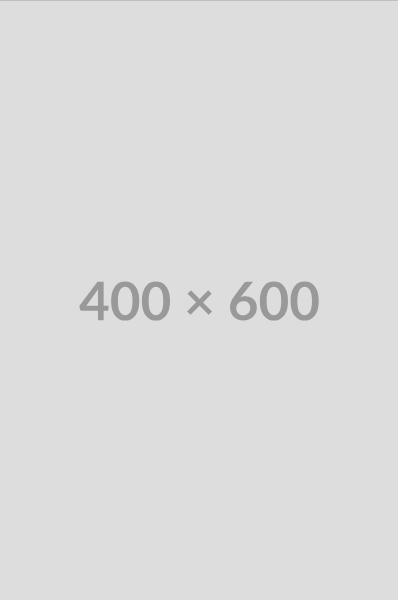
\includegraphics[width=\linewidth, height=5cm, keepaspectratio]{images/placeholder.png} % Generic Placeholder Image

\end{tabularx} % End of the outer table

\vspace{1.5ex} % Space after the personal data block
%{\noindent\rule{\linewidth}{0.4pt}}% Draw the horizontal rule AFTER the table
%\vspace{2ex}% Add space after the rule before the next section starts

% --- WORK EXPERIENCE SECTION ---
\rulesection{Berufserfahrung}

\cvsectionentry{03/2022 - heute} % Randomized Date Range
               {Innovate Solutions GmbH, München} % Randomized Company & Location
               {Softwareentwickler Cloud Services} % Randomized Title
               {% Randomized Bullet points
                 \item Konzeption und Entwicklung von Microservices für Cloud-Plattformen (AWS, Azure)
                 \item Implementierung von CI/CD Pipelines mit Jenkins und GitLab CI
                 \item Mitarbeit in agilen Projektteams (Scrum)
               }

\cvsectionentry{08/2019 - 02/2022} % Randomized Date Range
               {Data Dynamics AG, Hamburg} % Randomized Company & Location
               {Werkstudent Data Analysis} % Randomized Title
               {% Randomized Bullet points
                 \item Aufbereitung und Analyse von Geschäftsdaten mit Python (Pandas, NumPy)
                 \item Erstellung von Dashboards und Reports (Tableau)
                 \item Unterstützung bei der Datenbankadministration (SQL)
               }

% --- EDUCATION SECTION ---
\rulesection{Ausbildung}

\cvsectionentry{10/2019 - 07/2021} % Randomized Date Range
               {Technische Universität Beispielstadt} % Randomized Institution
               {Master of Science, Informatik} % Randomized Degree
               {% Randomized Bullet points
                 \item Schwerpunkt: Verteilte Systeme und Cloud Computing
                 \item Masterarbeit: "Performance-Analyse von Container-Orchestrierungs-Tools"
               }

\cvsectionentry{10/2016 - 09/2019} % Randomized Date Range
               {Hochschule Musterstadt} % Randomized Institution
               {Bachelor of Science, Wirtschaftsinformatik} % Randomized Degree
               {% Randomized Bullet points
                 \item Schwerpunkt: Software Engineering und Projektmanagement
                 \item Bachelorarbeit: "Entwicklung einer Webanwendung zur Projektzeiterfassung"
               }

\cveduentrysimple{09/2013 - 07/2016} % Randomized Date Range
               {ABC Ausbildungszentrum GmbH, Frankfurt} % Randomized Institution
               {Ausbildung zum Fachinformatiker, Anwendungsentwicklung} % Randomized Qualification

\cveduentrysimple{2013} % Randomized Date
                  {Mustermann Realschule, Köln} % Randomized Institution
                  {Mittlere Reife} % Standard Qualification

% --- SKILLS SECTION ---
\rulesection{Kenntnisse}

\cvskillentry{Programmiersprachen}{ % Randomized Category & Skills
    \item Python (Sehr gut)
    \item Java (Gut)
    \item SQL (Gut)
    \item JavaScript (Grundlagen)
    \item Bash (Grundlagen)
}
\cvskillentry{Technologien / Frameworks}{ % Randomized Category & Skills
    \item AWS, Azure
    \item Docker, Kubernetes
    \item Spring Boot
    \item React
    \item Git, Jenkins
}
\cvskillentry{Sprachen}{ % Randomized Category & Skills
    \item Deutsch (Muttersprache)
    \item Englisch (Verhandlungssicher, C1)
    \item Französisch (Grundlagen)
}
\cvskillentry{Betriebssysteme}{ % Randomized Category & Skills
    \item Linux (Ubuntu, Debian)
    \item macOS
    \item Windows
}

% --- INTERESTS SECTION ---
\rulesection{Interessen}

\noindent % Randomized Interests
Open Source Software, Automatisierung, Bergsport, Kochen, Reisen, Fotografie.

% --- DOCUMENT END ---
\end{document}